\documentclass[a4paper,14pt]{extarticle}

% Путь до папки с общими шаблонами
\newcommand{\pathToCommonFolder}{/home/denilai/Documents/repos/latex/Common}
% Название работы в титуле
\newcommand{\workname}{Отчет по практической работе №4}
% Название дисциплины в титуле
\newcommand{\discipline}{Системное программное обеспечение}
% Название кафедры в титуле
\newcommand{\kafedra}{Кафедра Математического обеспечения и стандартизации информационных технологий}
% Тема работы в титуле
\newcommand{\theme}{Системы конфигурационного управления}
\newcommand{\rang}{ассистент}
\newcommand{\teacherfio}{Ю.~А.~Вороноцов}



% установка размера шрифта для всего документа
%\fontsize{20pt}{18pt}\selectfont
\usepackage{extsizes} % Возможность сделать 14-й шрифт

\author{Кирилл Денисов}
\title{Практическая работа №3}
\date{\today}

% установка полуторного интервала
% \usepackage{setspace}  
% \onehalfspacing



% Вставка заготовки преамбулы
% Этот шаблон документа разработан в 2014 году
% Данилом Фёдоровых (danil@fedorovykh.ru) 
% для использования в курсе 
% <<Документы и презентации в \LaTeX>>, записанном НИУ ВШЭ
% для Coursera.org: http://coursera.org/course/latex .
% Исходная версия шаблона --- 
% https://www.writelatex.com/coursera/latex/5.3

% В этом документе преамбула

% Для корректного использования русских символов в формулах
% пакеты hyperref и настройки, связанные с ним, стоит загуржать
% перед загрузкой пакета mathtext



% поддержка русских букв
% кодировка шрифта
%\usepackage[T2A]{fontenc} 
\usepackage{pscyr}

% использование ненумеровонного абзаца с добавлением его в содержаниеl

\newcommand{\anonsection}[1]{\section*{#1}\addcontentsline{toc}{section}{#1}}
\newcommand{\sectionunderl}[1]{\section*{\underline{#1}}}


% настройка окружения enumerate
\usepackage{enumitem}
\setlist{noitemsep}
\setlist[enumerate]{labelsep=*, leftmargin=1.5pc}

\usepackage{hyperref}

% сначала ставить \usepackage{extsizes} % Возможность сделать 14-й шрифт
% для корректной установки полей вставлять преамбулу следует в последнюю очередь (но перед дерективой замены \rmdefault)
\usepackage[top=20mm,bottom=25mm,left=35mm,right=20mm]{geometry} % Простой способ задавать поля

\hypersetup{				% Гиперссылки
	unicode=true,           % русские буквы в раздела PDF
	pdftitle={Заголовок},   % Заголовок
	pdfauthor={Автор},      % Автор
	pdfsubject={Тема},      % Тема
	pdfcreator={Создатель}, % Создатель
	pdfproducer={Производитель}, % Производитель
	pdfkeywords={keyword1} {key2} {key3}, % Ключевые слова
	colorlinks=true,       	% false: ссылки в рамках; true: цветные ссылки
	linkcolor=red,          % внутренние ссылки
	citecolor=black,        % на библиографию
	filecolor=magenta,      % на файлы
	urlcolor=blue           % на URL
}

%%% Работа с русским языком
\usepackage{cmap}					% поиск в PDF
\usepackage{mathtext} 				% русские буквы в формулах
\usepackage[T2A]{fontenc}			% кодировка
\usepackage[utf8]{inputenc}			% кодировка исходного текста
\usepackage[english,russian]{babel}	% локализация и переносы
\usepackage{indentfirst}
\frenchspacing

%для изменения названия списка иллюстраций
\usepackage{tocloft}


\renewcommand{\epsilon}{\ensuremath{\varepsilon}}
\renewcommand{\phi}{\ensuremath{\varphi}}
\renewcommand{\kappa}{\ensuremath{\varkappa}}
\renewcommand{\le}{\ensuremath{\leqslant}}
\renewcommand{\leq}{\ensuremath{\leqslant}}
\renewcommand{\ge}{\ensuremath{\geqslant}}
\renewcommand{\geq}{\ensuremath{\geqslant}}
\renewcommand{\emptyset}{\varnothing}

% Изменения параметров списка иллюстраций
\renewcommand{\cftfigfont}{Рисунок } % добавляем везде "Рисунок" перед номером
\addto\captionsrussian{\renewcommand\listfigurename{Список иллюстративного материала}}

\newcommand{\tm}{\texttrademark\ }
\newcommand{\reg}{\textregistered\ }


%%% Дополнительная работа с математикой
\usepackage{amsmath,amsfonts,amssymb,amsthm,mathtools} % AMS
\usepackage{icomma} % "Умная" запятая: $0,2$ --- число, $0, 2$ --- перечисление

%% Номера формул
%\mathtoolsset{showonlyrefs=true} % Показывать номера только у тех формул, на которые есть \eqref{} в тексте.
%\usepackage{leqno} % Нумереация формул слева

%% Свои команды
\DeclareMathOperator{\sgn}{\mathop{sgn}}

%% Перенос знаков в формулах (по Львовскому)
\newcommand*{\hm}[1]{#1\nobreak\discretionary{}
{\hbox{$\mathsurround=0pt #1$}}{}}


% отступ для первого абзаца главы или параграфа
%\usepackage{indentfirst}

%%% Работа с картинками
\usepackage{graphicx}  % Для вставки рисунков
\graphicspath{{images/}{screnshots/}}  % папки с картинками
\DeclareGraphicsExtensions{.pdf,.png,.jpg}
\setlength\fboxsep{3pt} % Отступ рамки \fbox{} от рисунка
\setlength\fboxrule{1pt} % Толщина линий рамки \fbox{}
\usepackage{wrapfig} % Обтекание рисунков текстом

%%% Работа с таблицами
\usepackage{array,tabularx,tabulary,booktabs} % Дополнительная работа с таблицами
\usepackage{longtable}  % Длинные таблицы
\usepackage{multirow} % Слияние строк в таблице

%%% Теоремы
\theoremstyle{plain} % Это стиль по умолчанию, его можно не переопределять.
\newtheorem{theorem}{Теорема}[section]
\newtheorem{proposition}[theorem]{Утверждение}

\theoremstyle{plain} % Это стиль по умолчанию, его можно не переопределять.
\newtheorem{work}{Практическая работа}[part]


 
 
\theoremstyle{definition} % "Определение"
\newtheorem{corollary}{Следствие}[theorem]
\newtheorem{problem}{Задача}[section]
 
\theoremstyle{remark} % "Примечание"
\newtheorem*{nonum}{Решение}



%%% Программирование
\usepackage{etoolbox} % логические операторы

%%% Страница

%	\usepackage{fancyhdr} % Колонтитулы
% 	\pagestyle{fancy}
%   \renewcommand{\headrulewidth}{0pt}  % Толщина линейки, отчеркивающей верхний колонтитул
% 	\lfoot{Нижний левый}
% 	\rfoot{Нижний правый}
% 	\rhead{Верхний правый}
% 	\chead{Верхний в центре}
% 	\lhead{Верхний левый}
%	\cfoot{Нижний в центре} % По умолчанию здесь номер страницы

\usepackage{setspace} % Интерлиньяж
\onehalfspacing % Интерлиньяж 1.5
%\doublespacing % Интерлиньяж 2
%\singlespacing % Интерлиньяж 1

\usepackage{lastpage} % Узнать, сколько всего страниц в документе.

\usepackage{soul} % Модификаторы начертания


\usepackage[usenames,dvipsnames,svgnames,table,rgb]{xcolor}


\usepackage{csquotes} % Еще инструменты для ссылок

%\usepackage[style=authoryear,maxcitenames=2,backend=biber,sorting=nty]{biblatex}

\usepackage{multicol} % Несколько колонок

\usepackage{tikz} % Работа с графикой
\usepackage{pgfplots}
\usepackage{pgfplotstable}

% модуль для вставки рыбы
\usepackage{blindtext}

\usepackage{listings}
\usepackage{color}


% для поворота отдельной страницы. Использовать окружение \landscape
\usepackage{pdflscape} 
\usepackage{rotating} 


\definecolor{mygreen}{rgb}{0,0.6,0}
\definecolor{mygray}{rgb}{0.5,0.5,0.5}
\definecolor{mymauve}{rgb}{0.58,0,0.82}


% пример импорта файла
%\lstinputlisting{/home/denilai/repomy/conf/distributions}

\lstset{
	language=Python,
	basicstyle=\footnotesize,        % the size of the fonts that are used for the code
	numbers=left,                    % where to put the line-numbers; possible values are (none, left, right)
	numbersep=5pt,                   % how far the line-numbers are from the code
	numberstyle=\tiny\color{mygray}, % the style that is used for the line-numbers
	stepnumber=2,                    % the step between two line-numbers. If it's 1, each line will be numbered
	% Tab - 2 пробела
	tabsize=2,    
	% Автоматический перенос строк
	breaklines=true,
	frame=single,
	breakatwhitespace=true,
	title=\lstname 
}



% использовать Times New Roman
\renewcommand{\rmdefault}{ftm}

\begin{document}
	\thispagestyle{empty}
	
	% Вставка первого титульного листа
	%\newcounter{withouttheme}

%\setcounter{withouttheme}{<n>} установить значение счетчика  withouttheme для определения, нужна ли тема
%    {0} - нужна
%    {1} - не нужна

%\setcounter{withoutsubmissiondate}{<n>} установить значение счетчика  withoutsubmissiondate для определения, нужна ли дата представления к защите
%     {0} - нужна
%     {1} - не нужена
\begin{center}
	\begin{figure}[h!]
		\begin{center}
		%\vspace{-10ex}
		
\includegraphics[width=0.17\linewidth]{\pathToCommonFolder/gerb}
		%\caption{}\label{pic:first}
		%	\vspace{5ex}
		\end{center}	
	\end{figure}
 	\small	МИНОБРНАУКИ РОССИИ \\
	Федеральное государственное бюджетное образовательное учреждение\\
						высшего образования\\
\normalsize					
\textbf{«МИРЭА – Российский технологический университет»\\
						РТУ МИРЭА}\\
						\noindent\rule{1\linewidth}{1pt}\\
       Институт информационных технологий\\ %\vspace{2ex}
					\kafedra\\
		\vspace{3ex}
			\large \textbf{\workname}  \\
		%\vspace{1ex}
						по дисциплине\\ «\discipline» \\
		\vspace{3ex}
		\ifnum \value{withouttheme}=0 {
			\textbf{Тема работы:}\\ <<\theme>>
		}
		\else {}
		\fi
\vspace{10ex}
\small
\begin{table}[h!]
\begin{tabular}{lp{0.6\linewidth}l}
	\textbf{Выполнил:} & студент группы ИВБО-02-19 & \\ 
	& & \studentfio \\%Д.~Н.~Федосеев\\%А.~М.~Сосунов\\%К.~Ю.~Денисов\\%И.~А.~Кремнев
	\textbf{Принял:} & \rang & \\
	& & \teacherfio \hfill\\
\end{tabular}
\end{table}
\end{center}
\ifnum \value{withoutsubmissiondate}=0 {
	\begin{flushleft}
		Работа представлена к защите <<\rule{3ex}{1pt}>>\rule{10ex}{1pt} 202\rule{1ex}{1pt} г.\hfill
	\end{flushleft}
\else {}
\fi

\normalsize
\begin{center}	
\vfill
Москва 2022
\end{center}

	
	\newpage
	\tableofcontents
	\newpage

\section{Подготовка инфраструктуры}
В ходе данной практической работы мы будем использовать три виртуальные машины под управлением ОС GNU/Linux Debian 8.3.0, одна из которых будет управляющей и будет выполнять конфигурацию и настройку двух управляемых машин.

Настроим ip-адрес управляемых машин. См рисунки \ref{img:interfaces1} и \ref{img:interfaces2} в \hyperref[A]{Приложении А}.
Установим \textbf{ansible} и сервер \textbf{ssh} на управляющую машину. См. рисунок \ref{img:ansi-version} и \ref{img:ssh-version}.

Настроим inventory-файл:

\lstinputlisting{/home/denilai/Desktop/hosts}
После установки данных сервисов, проверим возможность подключения по ssh, предварительно сгенерировав ключи командой \textbf{ssh-keygen} и передав их на управляемые машины командами:
\begin{lstlisting}
$ ssh-copy-id root@192.168.43.101
$ ssh-copy-id root@192.168.43.201
\end{lstlisting}
Cм. рисунок \ref{img:ssh-root}.

Выполним следующий команды для проверки работы ansible:
\begin{lstlisting}
$ ansible -i ./hosts -m ping all
$ ansible -i ./hosts -m command -a free all
\end{lstlisting}
См. рисунок \ref{img:ansi-commands}.

\section{Использование Ansible для конфигурации хостов}

Напишем playbook, который установит веб-сервер Nginx на управляемые хосты.
\lstinputlisting{/home/denilai/Desktop/playbook-nginx.yml}

Выполним данную команду для выполнения playbook-а.
\begin{lstlisting}
$ ansible-playbook -i hosts playbook-nginx.yml
\end{lstlisting}


После выполнения playbook-а, проверим статус \textbf{nginx} на первой управляемой машине. См. рисунки \ref{img:playbook-nginx.yml} и \ref{img:nginx-status-1}.

\newpage
\section{Более сложный playbook}
Приведем содержание более сложного playbook-а:
\lstinputlisting{/home/denilai/Desktop/playbook-param-nginx.yml}

Теперь выполним команду для запуска playbook’а с пробным прогоном, который позволит проверить корректность написанного playbook’а без внесения изменений на целевые узлы.

\begin{lstlisting}
$ ansible-playbook -i hosts playbook-param-nginx.yml --check
\end{lstlisting}
Результат проверки можно увидеть на рисунке \ref{img:playbook-param-check}.

После удачной проверки, выполним playbook, исключив из команды ключ \textbf{--check}, а затем запросим базовую страницу при помощи утилиты curl. См. рисунок \ref{img:playbook-param}.

\section{Роли Ansible}

Попробуем создать свою роль для установки ранее разобранного playbook’а nginx. Сперва вернёмся в рабочую папку со всеми файлами для Ansible и создадим там директорию \textbf{roles}. После чего перейдём в эту директорию и инициируем роль стандартной структуры при помощи данной команды:
\begin{lstlisting}
$ ansible-galaxy init nginx
\end{lstlisting}

При помощи команды \textbf{tree} можно опять же посмотреть структуру директории.

Перейдём к созданию роли. Заполним соответствующие файлы данными из секций playbook’а и соответствующие директории ранее созданными файлами.

Теперь напишем playbook, запускающий созданную роль. Для вызова составленной роли в playbook’е используется секция \textbf{roles}. Создадим файл \textbf{nginx-role.yml} в рабочей директории ansible и заполним его следующим образом.

\lstinputlisting{/home/denilai/Desktop/nginx-role.yml}

После этого выполним данный playbook на первом сервере. См. рисунок \ref{img:nginx-role}.

\section{Индивидуальное задание}
В качестве индивидуального задания для \textbf{варианта 6} предлагается написать роль для сервера \textbf{nginx}, написать playbook для применения роли, провести тестовый запуск playbook’а, в случае успешного прохождения теста, применить playbook к серверам.

Необходимо добавить переменную, содержащую ФИО, номер группы и номер варианта. 

Данная переменная должна выводиться в шаблонный файл nginx.
Установка пакета выполняется при помощи модуля \textbf{APT}, используемого для установки \textbf{nginx} в базовой роли.

\lstinputlisting{/home/denilai/Desktop/nginx-role-sql.yml}
Добавим еще одну секцию в файл /tasks/main.yml, чтобы установить пакет клиента базы данных MySql.
\begin{lstlisting}
 - name: Install Mysql client
apt:
name=default-mysql-client
state=present
update_cache=yes
\end{lstlisting}

Изменим содержание файла \textbf{hello.html.j2} --- добавим ФИО студента и номер варианта.
\lstinputlisting{/home/denilai/Desktop/hello.html.j2}

Протестируем корректность составления роли, выполнив следующую команду:
\begin{lstlisting}
$ ansible-playbook -i ./hosts nginx-role-sql.yml --check
\end{lstlisting}
См. рисунок \ref{img:nginx-role-sql}.

Применим playbook к серверам. См. рисунок См. рисунок \ref{img:nginx-role-sql1}. Далее проверим содержание созданной при помощи шаблона страницы \textbf{hello} с помощью данной команды:
\begin{lstlisting}
$ curl -L http://192.168.43.101/hello
\end{lstlisting}
См. рисунок \ref{img:hello-nginx}.


\section{Вывод}
В результате выполнения данной практической работы мы научились
использовать систему конфигурационного управления Ansible. Написали playbook для применения роли для сервера nginx, протестировали его работу.

\newpage
{\centering
\anonsection{ПРИЛОЖЕНИЕ А}
}
\label{A}
\begin{figure}[hptb]
	\centering
	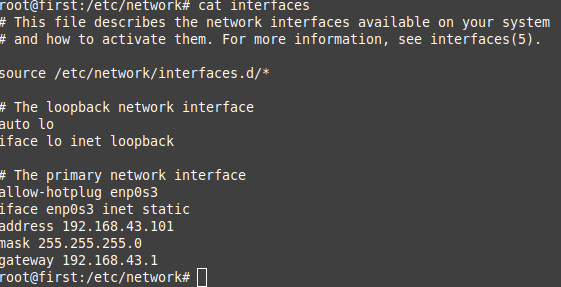
\includegraphics[width=0.8\linewidth]{interfaces1}
	\caption{Файл /etc/networks/interfaces 1-ой машины}
	\label{img:interfaces1}
\end{figure}

\begin{figure}[hptb]
	\centering
	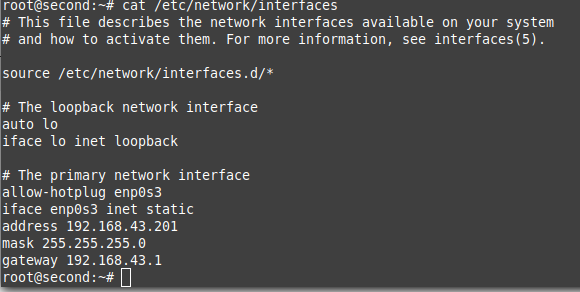
\includegraphics[width=0.8\linewidth]{interfaces2}
	\caption{Файл /etc/networks/interfaces 2-ой машины}
	\label{img:interfaces2}
\end{figure}
\newpage


\begin{figure}[hptb]
	\centering
	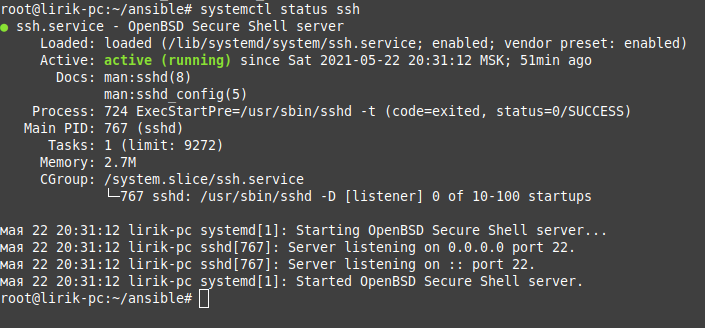
\includegraphics[width=0.8\linewidth]{ssh-version}
	\caption{Версия сервера ssh}
	\label{img:ssh-version}
\end{figure}
%\newpage
\begin{figure}[hptb]
	\centering
	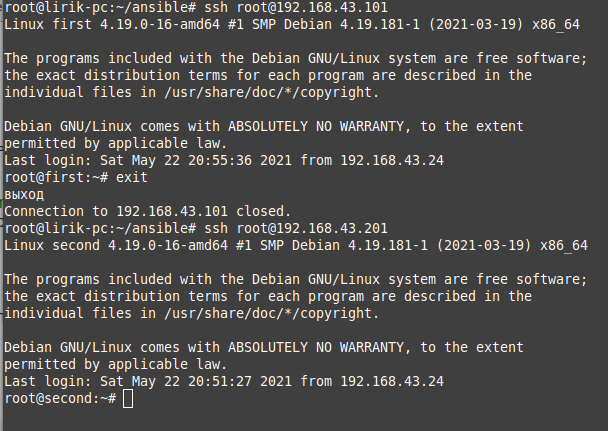
\includegraphics[width=0.7\linewidth]{ssh-root}
	\caption{Подключение к машинам}
	\label{img:ssh-root}
\end{figure}
\newpage
\begin{figure}[hptb]
	\centering
	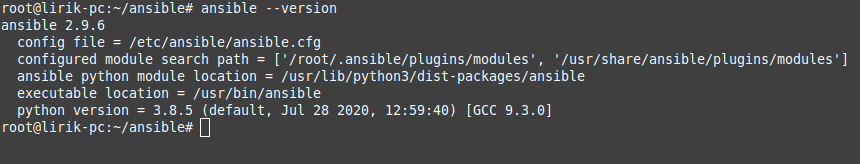
\includegraphics[width=0.8\linewidth]{ansi-version}
	\caption{Версия ansible}
	\label{img:ansi-version}
\end{figure}

\begin{figure}[hptb]
	\centering
	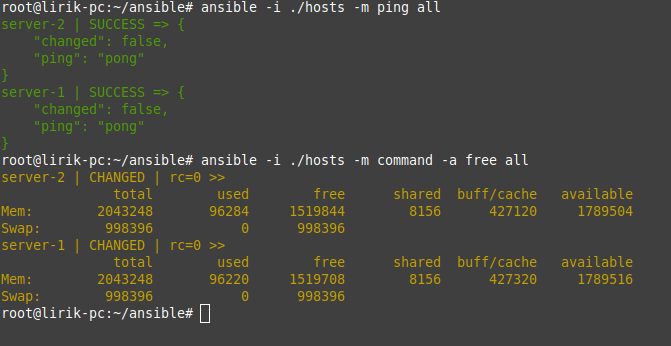
\includegraphics[width=0.8\linewidth]{ansi-commands}
	\caption{Простые команды}
	\label{img:ansi-commands}
\end{figure}

\begin{figure}[hptb]
	\centering
	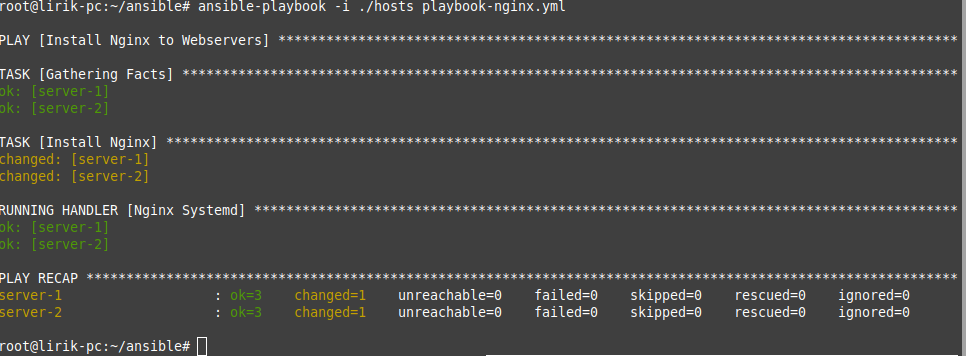
\includegraphics[width=0.8\linewidth]{playbook-nginx}
	\caption{Простой playbook}
	\label{img:playbook-nginx.yml}
\end{figure}
\newpage
\begin{figure}[hptb]
	\centering
	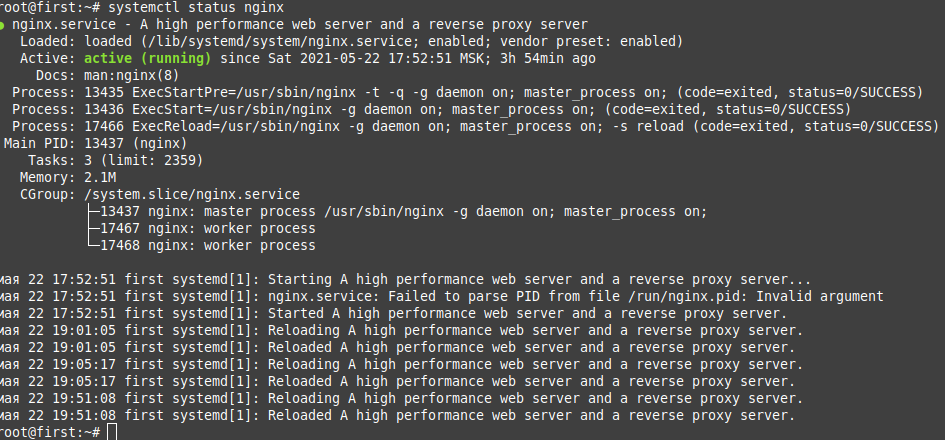
\includegraphics[width=0.8\linewidth]{nginx-status-1}
	\caption{Статус nginx}
	\label{img:nginx-status-1}
\end{figure}

\begin{figure}[hptb]
	\centering
	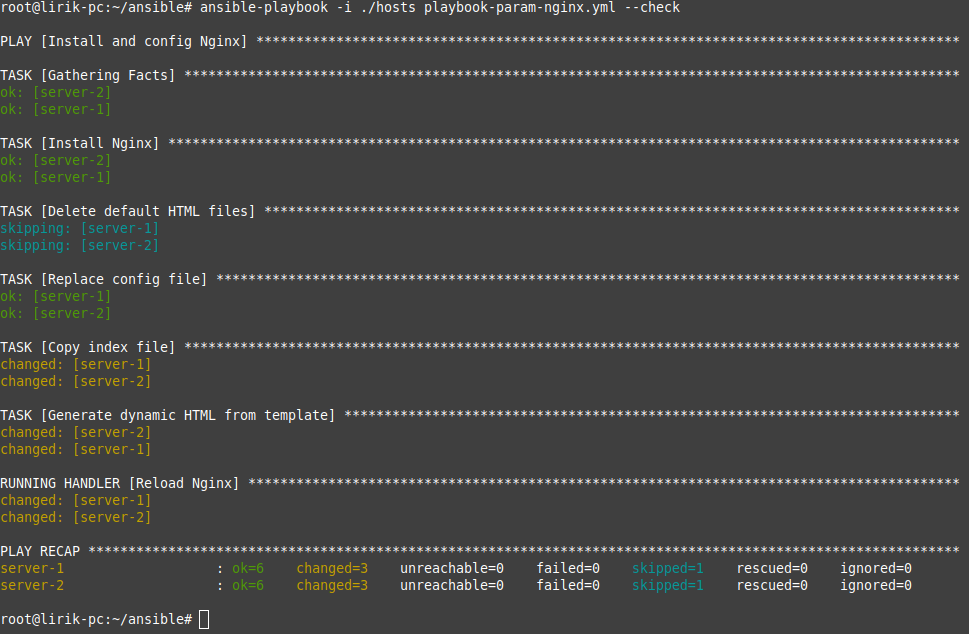
\includegraphics[width=0.8\linewidth]{playbook-param-check}
	\caption{Проверка сложного playbook-а}
	\label{img:playbook-param-check}
\end{figure}
\newpage
\begin{figure}[hptb]
	\centering
	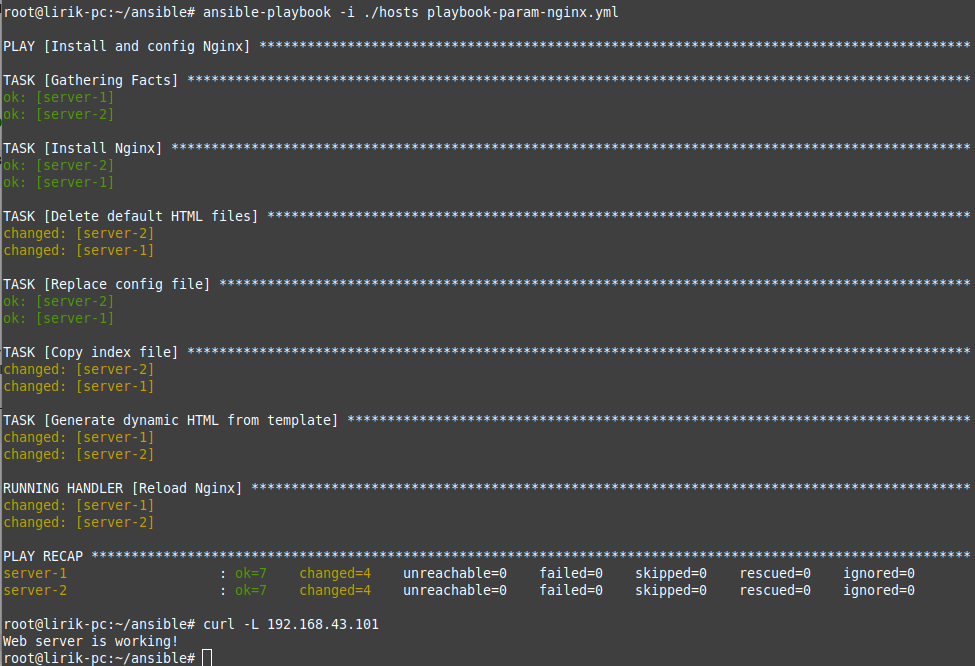
\includegraphics[width=0.7\linewidth]{playbook-param}
	\caption{Запуск сложного playbook-а}
	\label{img:playbook-param}
\end{figure}

\begin{figure}[hptb]
	\centering
	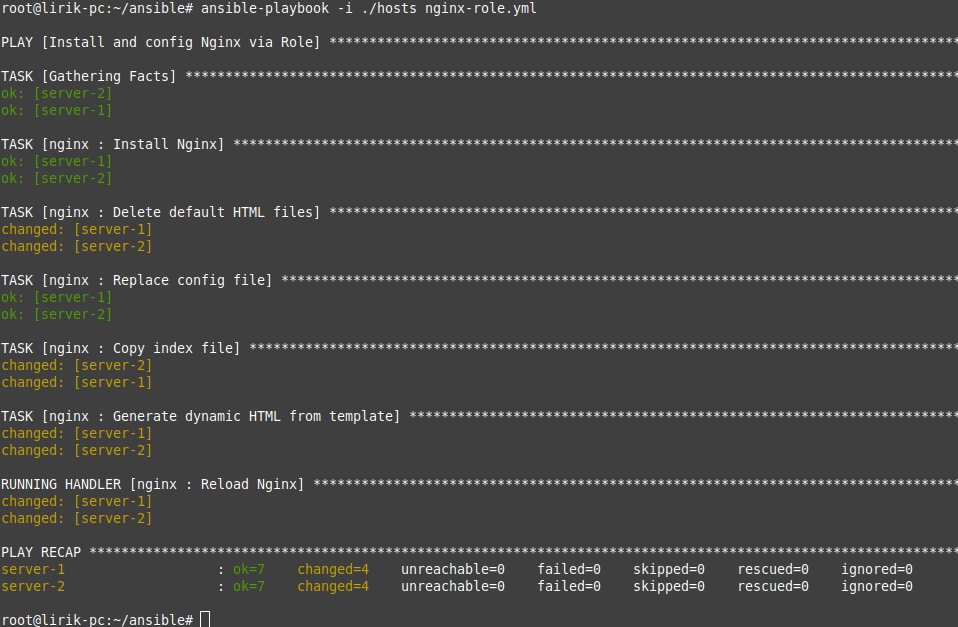
\includegraphics[width=0.7\linewidth]{nginx-role}
	\caption{Запуск playbook-а с ролью}
	\label{img:nginx-role}
\end{figure}

\begin{figure}[hptb]
	\centering
	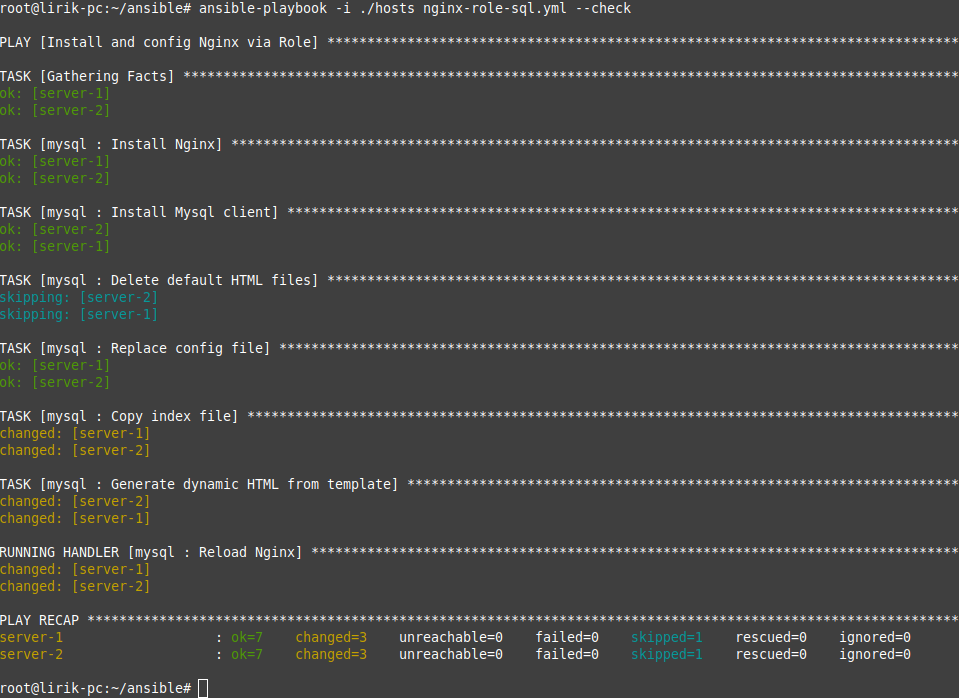
\includegraphics[width=0.7\linewidth]{nginx-role-sql}
	\caption{Проверка индивидуального playbook-а с ролью}
	\label{img:nginx-role-sql}
\end{figure}

\begin{figure}[hptb]
	\centering
	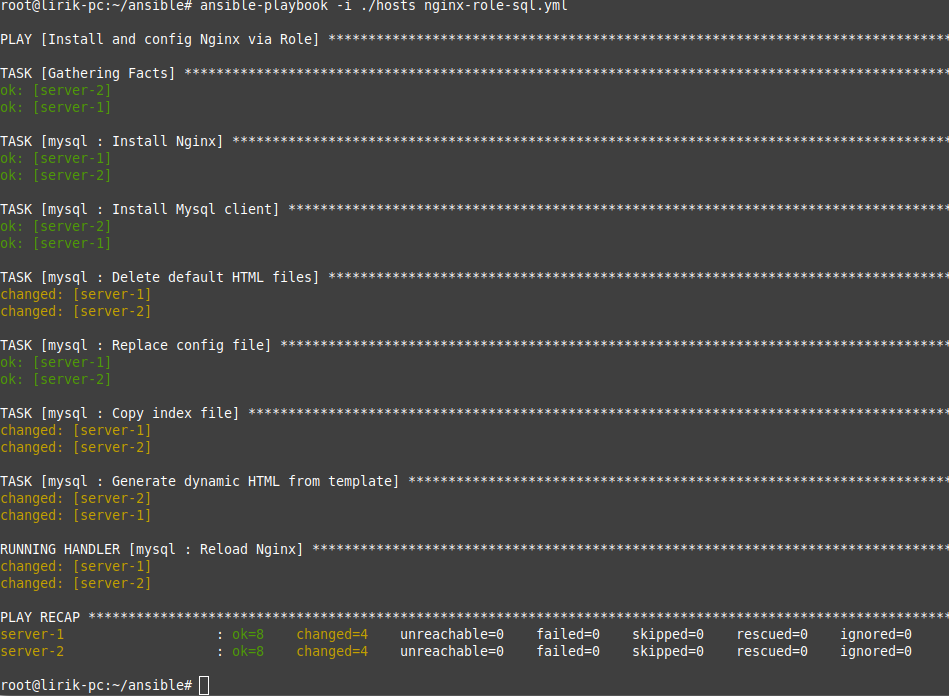
\includegraphics[width=0.7\linewidth]{nginx-role-sql1}
	\caption{Запуск индивидуального playbook-а с ролью}
	\label{img:nginx-role-sql1}
\end{figure}

\begin{figure}[hptb]
	\centering
	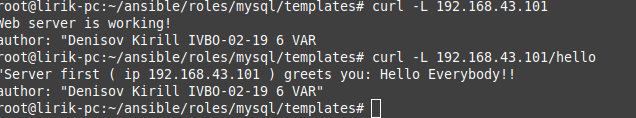
\includegraphics[width=0.7\linewidth]{hello-nginx}
	\caption{Страница hello}
	\label{img:hello-nginx}
\end{figure}


\end{document}
